\documentclass[../ComputerNetworks.tex]{subfiles}

\usepackage{hyperref}
\usepackage{graphicx}

\hypersetup{
  colorlinks=true,
  citecolor=cyan,
  linkcolor=magenta,
  urlcolor=blue}

\begin{document}

\subsection{Introduzione}

L’obbiettivo del \textbf{PSTN} (\textbf{Public Switched Telephone Network}) é trasmettere la voce umana per lunghe distanze in maniera riconoscibile.
Le problematiche da affrontare sono molteplici, tra cui l’organizzazione della stesura dei cavi per offrire il servizio ad ogni casa.
Data l’evidente impossibilitá di far passare cavi individualmente che connettono ogni cliente all’altro, é stato sviluppato un sistema in grado di ridurre il numero di cavi da installare, permettendo il servizio a tutti senza restrizioni.
Sono stati quindi utilizzati cavi ad alta bandwidth e infrastrutture di multiplexing.

Tra gli uffici della compagnia telefonica la comunicazione avviene a banda elevata (fibra ottica), mentre all’"ultimo miglio" sono usati cavi di rame appartenenti alla telefonia.
Con il tempo questi vecchi impianti verranno sostituiti con attrezzature progettate per la trasmissione di dati.

\subsection{Struttura del sistema telefonico}

\begin{figure}[h]
    \centering
    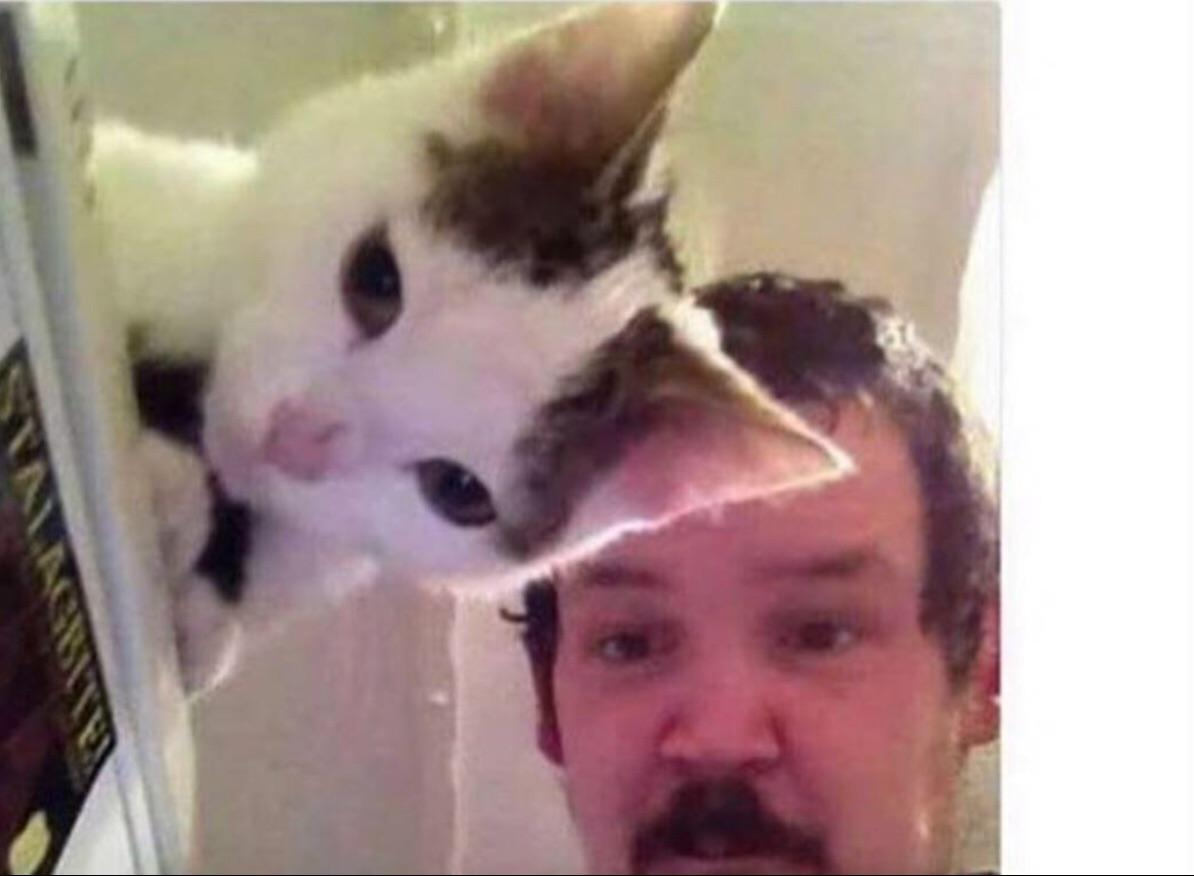
\includegraphics[width=0.5\textwidth]{img/29.jpg}
    \caption{(a) Fully interconnectrd network. (b) Centralized switch. (c) Two-level hierarchy}
    \label{fig29}
\end{figure}

Quando Bell brevettò il telefono, questo tipo di servizio era molto richiesto ed era a carico del cliente l’installazione del cavo per permettere la comunicazione.
Se un cliente voleva parlare con \emph{n} altri clienti allora ogni proproprietario doveva collegarsi con \emph{n} cavi ad ognuno\ref{fig29}(a).
Maggiori sono i clienti maggiore é il numero di cavi, trasformando le cittá in un groviglio di cavi che passavano sopra ogni albero.

Questo tipo di modello per connettere i clienti non era adeguato, cosí la Bell Telephone Company aprí il primo switching office.
La compagnia collegava ogni cliente al suo uffico, al cui interno degli operatori connettono coloro il chiamante al chiamato.

Ben presto, ogni cliente voleva fare chiamate a lunga distanza e ogni ufficio fu collegato ad ogni ufficio delle cittá vicine\ref{fig29}(b), riproponendo il problema indicato in \ref{fig29}(a).
Cosí la compagnia introdusse una gerarchia a due livelli\ref{fig29}(c).

Semplificando, ogni telefono é collegato direttamente all’\textbf{end office} (\textbf{local central office}) piú vicino, ad una distanza da 1 a 10 km.
Il collegamento tra ogni cliente e l’end office é chiamato \textbf{local loop}\footnote{Nel 1890, 80\% del capitale di AT\&T era il rame costrituente i local loop d’America}.

Se un cliente di un dato end office chiama una altro cliente appartenente allo stesso end office, il meccanismo di switching connette direttamente (corto circuito) i due local loop.

Se un cliente chiama un altro appartenente ad un altro end office, il meccanismo é diverso.
Ogni end office ha un numero di linee uscenti, chiamate \textbf{toll connecting trunks}, che collega agli uffici vicini, che sono chiamate \textbf{toll officies} o se sono nella stessa area \textbf{tandem officies}.

Se il chiamante e il chiamato sono collegati da un toll office comune, allora la connessione é stabilita all’interno dello stesso toll office, altrimenti deve essere stabilita un connessione tra almeno due toll officies.
I toll officies comunicano attraverso \textbf{intertoll trunks} (o \textbf{interoffice trunks}) ad banda elevata.
Fino allo scioglimento dell’AT\&T, la connessione tra toll officies era stabilita attraverso un sistema gerarchico di instradamento, dopo di che é stato sostituito da un sistama non-gerarchico piú flessibile (figura \ref{fig:nger}).

\begin{figure}[h]
    \centering
    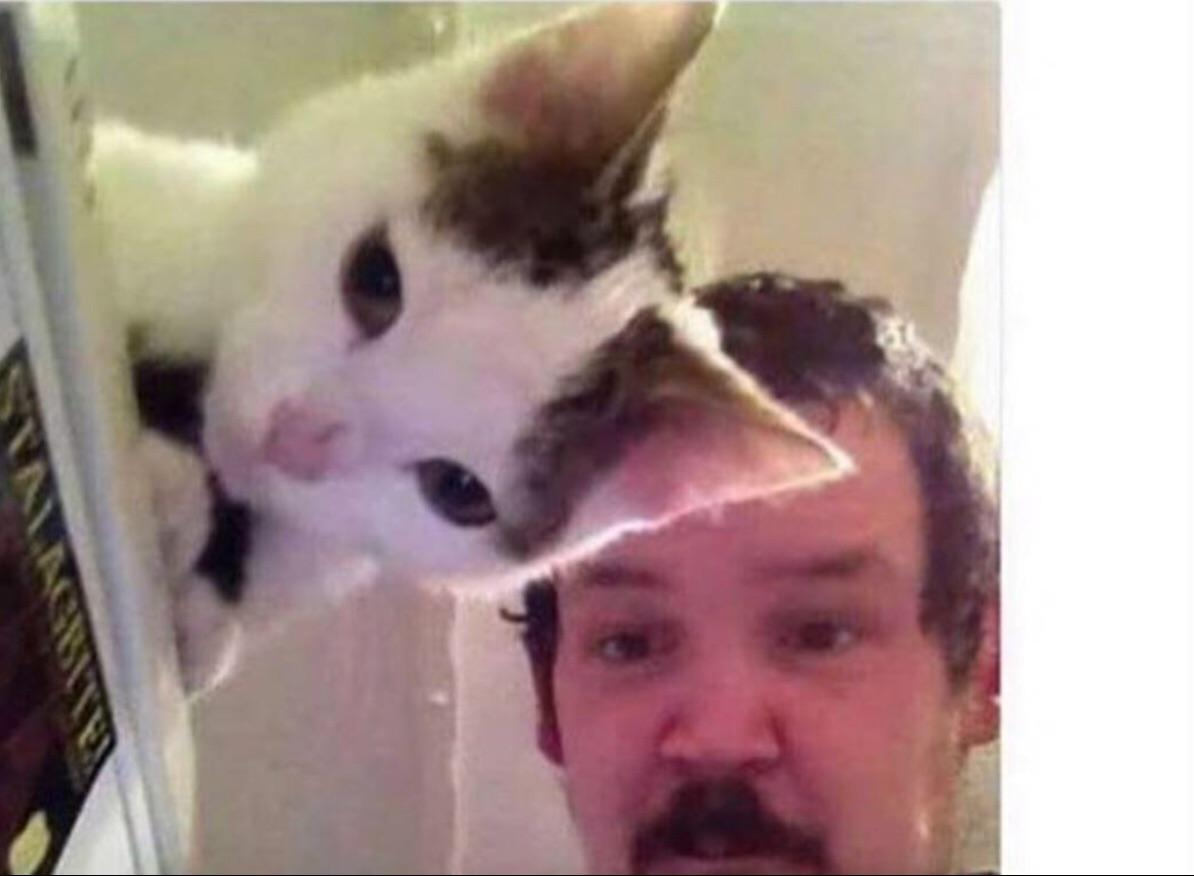
\includegraphics[width=0.5\textwidth]{img/30.jpg}
    \caption{A typical ciucuit route for long-distance call}
    \label{fig:nger}
\end{figure}

Con il passare del tempo, la trasmissione si è evoluta da analogia a digitale, sino ai nostri giorni, in cui l'unica parte ancora analogica è il local loop.

Il digitale è preferito perchè non è necessario riprodurre accuratamente il segnale analogico per comunicare l'informazine, anche se passa per più amplificatori lungo il suo cammino.
Ciò lo rende più affidabile e meno costosa e più facile da mantenere.

Riassumendo, il sistema telefonico consiste in:
\begin{itemize}
    \item Local loop: analog twisted pairs going to houses and business.
    \item Trunks: digital fiber optic links connecting switching officeis.
    \item Switching offices: where calls are moved from one trunk to another.
\end{itemize}

% Introdusse così una gerarchia a due livelli di switching toll (uffici interurbani).

\subsection{The local Loop: Modems, ADSL, and Fiber}

Con "Local Loop"\footnote{Anche conosciuto come "last mile" (ultimo miglio).} si intende come è strutturato l'infrastruttura dalla cabina dell'ISP fino al DSL-Client.
\'E la connessione fisica o circuito che connette dai public switched telephone network alle attrezzature adibite alla connessione degli usofruitori del servizio di dati.

Il problema consiste che, a prescindere della bandwidth che ha a disposizione la DSLAM, la linea tra la centralina e la residenza del cliente è, nella maggior parte dei casi, la stessa linea telefonica che è limita in frequenza.
Tecnologie come \emph{ADSL}, riutilizzano la linea telefonica già presente.
Però la linea telefonica è stata progettata per trasmettere la voce umana per il telefono in analogico e quindi ha caratteristiche che non sono adatte alla trasmissione di dati digitali a banda elevata.

Sia i modem che le \emph{ADSL} devono tener conto delle limitazioni dei vecchi impianti telefonici.

Di recente si stanno adoperando misure per installare fibre ottiche adatte alla trasmissione a banda larga.

\subsection{Telephone Modems}

Per inviare bits in un generico canale fisico, devono essere convertiti in segnali analogici che possono essere trasmessi attraverso il canale, attraverso delle tecniche di modulazione digitale.
A destinazione, questi segnali trasmessi saranno poi convertiti nuovamente da analogici a bits.

Il dispositivo che esegue la conversione dei flussi di dati in analogico e in digitale, è chiamato \textbf{modem} che sta per "\emph{mo}dulator \emph{dem}odulator".

I modem telefonici sono utilizzati per mandare bits tra due computer collegati tra di loro attraverso una linea telefonica adibita alla trasmissione della voce.

La linea telefonica è limitata a trasmettere a frequenza di 3100Hz, sufficienti a trasmettere una conversazione.
Per contestualizzare, la bandwidth dello standard Ethernete o 802.11 è quattro ordini di grandezza superiore.

Per il teorema di Nyquist, perfino per una linea perfetta a 3000Hz, non è possibile trasmettere a più di 6000 baud.
In pratica, la maggior parte dei modem, manda ad una frequnza di 2400 baud, trasmettendo bits multipli per simbolo, permettendo traffico comunicazione Full Duplex\footnote{usando frequenze differenti per direzioni differenti}.

Questi modem utilizzano 0 volts per trasmettere segnale logico 0 e 1 volt per segnale logico 1, con 1 bit per simbolo.
Un avanzamento è usare quattro simboli differenti come attraversi QPSK, cosicché si abbia 2 bit/symbol e raggiungere una frequenza di trasmissione di 4800 bps.

Frequenze di trasmissione maggiori necessitano insiemi di simboli\footnote{in gergo \textbf{costellation}} più ampi; ciò però significa anche che perfino una piccola quantità di rumore di fondo nel rilevamento di ampiezza o fase può produrre errori.

Prima dell'avvento delle connesioni 56k, il limite di bandwidth era di 35-kbps dovuto alla presenza di local loop alle estremità dell'infrastruttura di trasmissione, uno dalla parte degli end office (uffici di distribuzione locali dei servizi) e i Digital Subscriber.

L'approccio intrapreso per le connessioni 56-kbps, consiste nel rimuovere il local loop, tipicamente quello che lega ISP e l'end office più vicino, e sostituirlo con una linea di alta qualità e bandwidth.

Le linee telefoniche sono state progettate per trasmettere in analogico la voce umana

Ogni canale telefonico ha 4000Hz\footnote{per maggiori informazioni si guardi \href{https://en.wikipedia.org/wiki/Voice_frequency}{Voice Frequency}} di capacità, includendo le guard bands.
Per poter ricostruire il segnale trasmesso attraverso la linea, sono necessari 8000 campioni al secondo, per questa data frequenza\footnote{per il teorema di Nyquist}.
\'E stato scelto, come standard,  il numero di 8 bit al secondo per campione di cui uno per ragioni di controllo; ciò permette il trasferimento di 56000 bit/sec.

\subsection{Digital Subscriber Lines}

Il motivo per cui i modem appena discussi erano lenti, è dovuto al limite tecnico della linea per il quale è stato ottimizzata tutto il sistema, ovvero per trasmettere la voce umana.

Nel punto in cui ogni local loop termina in un end office, il cavo è collegato ad un filtro che attenua ogni frequenza sotto i 300Hz e sopra i 3400Hz\footnote{il cutoff non è netto per cui si considera 4000Hz}.

Nel caso di una \emph{xDSL}\footnote{nome generico utilizzato per un generico Digital Subscriber LIne} il customer è collegato in un altro tipo di switch che non ha il filtro integrato, permettendo di utilizzare a pieno la capacità del local loop.
Il fattore limitante rimane ora il local loop che supporta circa 1MHz.

Peró la capacitá del local loop diminuisce rapidamente all’aumentare della distanza dall’end office ed é dipendente anche dalla qualitá delle twisted pairs e dalla dimensione del cavo.

% fig33
\begin{figure}[h]
    \centering
    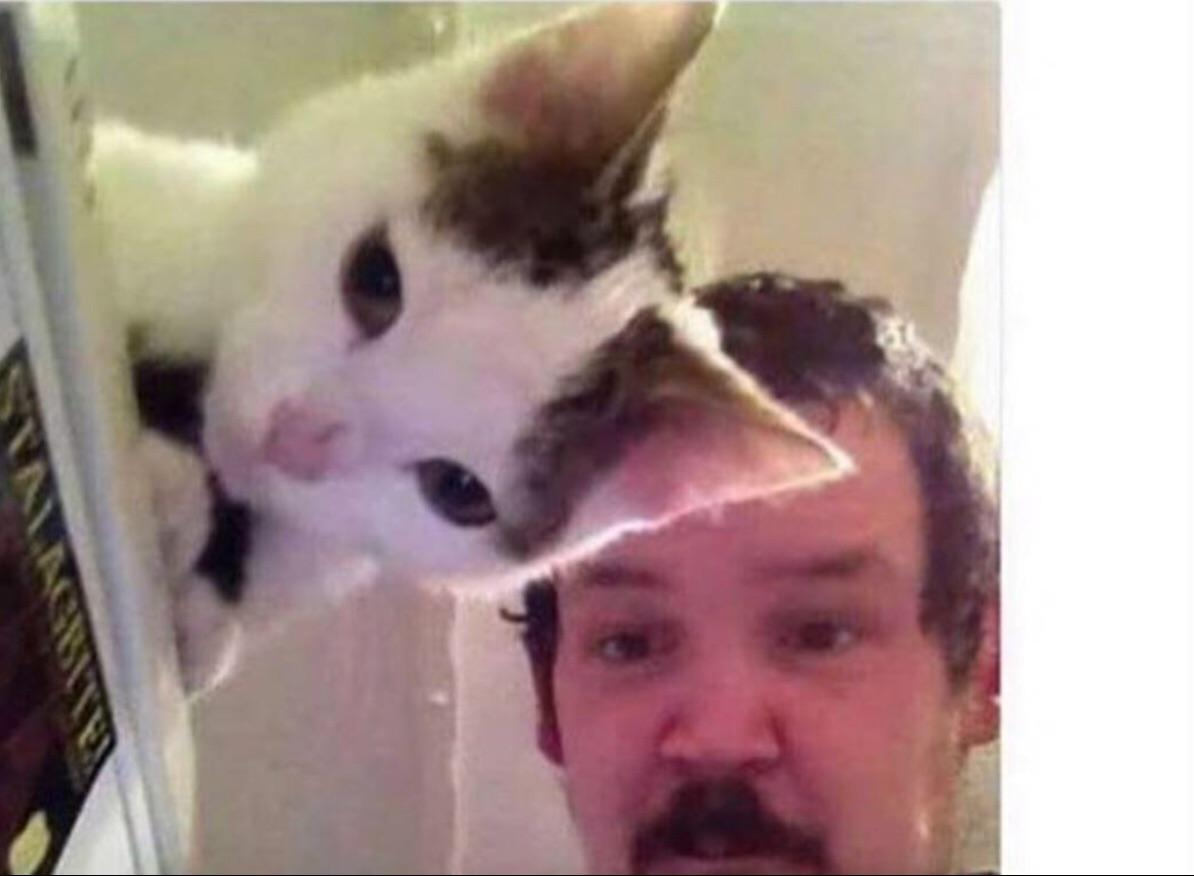
\includegraphics[width=0.5\textwidth]{img/distance.jpg}
    \caption{Bandwidth versus distance ocer Category 4UTP for DSL.}
\end{figure}

Ció implica che se si vuole garantire un servizio a velocitá minima, si é limitati in un raggio intorno all’end office, oltre il quale il servizio si degrada e non puó fornire le caratteristiche minime che si é imposto.
Minore é la velocitá scelta, maggiore é il raggio di copertura del servizio e maggiore é il numero di clienti coperti.
Ma minore é la velocitá e minore é invitante il servizio per cui i clienti dovrebbero pagare.

La \emph{xDSL} é stata progettata con determinati obbiettivi:
\begin{itemize}
    \item deve poter lavorare con l’infrastruttura corrente di Category 3 twisted pair local loops,
    \item non deve alterare il servizio telefonico e fax giá presente,
    \item deve essere piú veloce di 56kbps,
    \item deve avere un costo di mensile fisso e non per minuti di utilizzo.
\end{itemize}

Lo spettro di 1.1MHz é diviso in 256 canali indipendenti a livello del local loop.
Il canale 0 é utilizzato per il \emph{POTS} (Plain Old Telephone Service), i canali 1-5 sono inutilizzati per permettere che la voce e i dati non interferiscano tra di loro.
Tutti i rimanenti canali sono disponibili per la trasmissione dei dati e sono ripartiti in Upstream e Downstream.

Teoricamente tutti i canali potrebbero essere utilizzati in full-duplex, ma sperimentalmente il sistema garantisce velocitá molto inferiori.
Si é optato quindi di dividere i canali per poter garantire un servizio di qualitá maggiore.
Un rapporto di 50\% upstream e 50\% downstream é chiamato simmetrico, ma tipicamente il rapporto é sbilaciato a favore del downstream per necessitá dello stesso cliente; in questo caso di parla quindi di \emph{ADSL} dove la "A" corrisponde proprio ad "asimmetrico".

\begin{figure}[h]
    \centering
    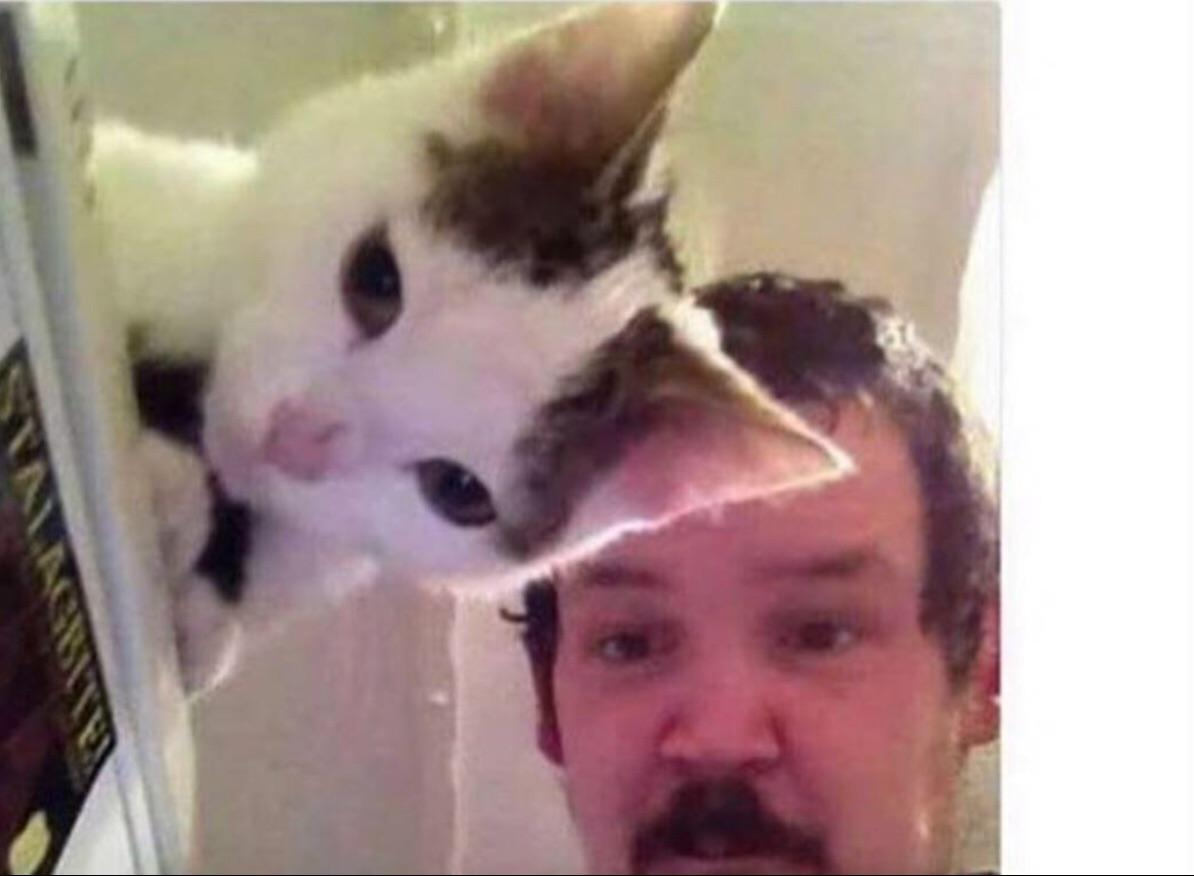
\includegraphics[width=0.5\textwidth]{img/ADSLeq.jpg}
    \caption{Typical ADSL equipment configuration. P44.}
\end{figure}

Per funzionare correttamente, la compagnia telefonica deve mandare un tecnico a installare un \textbf{NID} (\textbf{Network Interface Device}) nell’edificio del cliente.
Questo dispositivo marca la fine della proprietá della compagnia telefonica e la proprietá del cliente.
Vicino al NID (a volte é integrato all’interno) é presente un \textbf{splitter}, un filtro analogico che separa la banda 0-4000Hz adibita al POTS dai dati.
Il segnale del POTS é indirizzato verso l’impianto esistente del telefono e del fax, mentre i dati vengono indirizzati al modem ADSL, che usa digital signal processing per implementare OFDM.
Dato che la maggior parte dei modem é esterno, i computer devono essere connessi ad esso tramite un interfaccia ad alta velocitá come Ethernet, USB o 802.11(WIFI).

Nell’end office, é installato un corrispondente splitter, il quale, a sua volta, filtra la voce dai dati e li incammina verso il voice switch.
I dati superiori a 26kHz sono instadati al \textbf{DSLAM} (\textbf{Digital Subscriber Line Access Muptiplexer}), che processa il segnale in analogico e ricostruice i paccetti in digitale e li invia al ISP.

La separazione tra voce e ADSL, attraverso lo stesso tipologia di cavo, é relativamente poco costosa e necessita solo l’aggiunta di splitter e DSLAM (per servizi a banda bassa come all’utente casalingo).
Uno svantaggio di questo design, é che necessita di un NID e uno splitter per ogni cliente, il che necessita personale tecnico che vada ad installare i dispositivi casa per casa.

Un alternativa é usare lo standard \textbf{G.lite} che non necessita di splitter e utilizza la linea telefonica cosí comé.
Necessita peró di un microfiltro ad ogni telefono e non permette un velocitá simili alla tradizionale ADSL.

\subsection{Fiber To The Home}





\biblio
\end{document}
